\documentclass[10pt]{article}
\usepackage[utf8]{inputenc}
\usepackage{titlesec}

\title{\Huge \textbf{Relatório Final - Protocolos de Comunicação}}
\author{
Victor Miguel de Morais Costa (vmmc2) \\
Zilde Souto Maior Neto (zsmn)
}
\date{}

%%%%%%%%%%%%%%%%%%%%%%%%%%%%%%%%%%%%
\usepackage[colorlinks=true,allcolors=blue]{hyperref}
\usepackage{natbib}
\usepackage{graphicx}
\usepackage[brazilian]{babel}

\usepackage[a4paper,bindingoffset=0.2cm,%
            left=3cm,right=3cm,top=3cm,bottom=3cm,%
            footskip=.65cm]{geometry}
%%%%%%%%%%%%%%%%%%%%%%%%%%%%%%%%%%%%
\begin{document}
\maketitle
%%%%%%%%%%%%%%%%%%%%%%%%%%%%%%%%%%%%

\section{Introdução}
    \begin{itemize}
    \item O presente documento tem como objetivo: relatar, de forma detalhada, o processo de desenvolvimento da biblioteca que implementa protocolo a ser usado no projeto final da disciplina.
    \end{itemize}

\section{Objetivo}
    \begin{itemize}
    \item O protocolo foi elaborado com o objetivo de ser utilizado em um sistema de votação seguro em uma rede Wi-Fi não-confiável.
    \end{itemize}

\section{Decisões Iniciais de Implementação}
    \begin{itemize}
    \item Para o desenvolvimento da biblioteca responsável por implementar o protocolo em questão, foram tomadas algumas decisões técnicas e conceituais importantes:
        \begin{itemize}
        \item A biblioteca que implementa o protocolo foi desenvolvida na linguagem Python por questões de simplicidade e familiaridade dos integrantes.
        \item A biblioteca foi desenvolvida para sistemas operacionais Linux.
        \item Além disso, o protocolo, implementado pela biblioteca, foi desenvolvido segundo a arquitetura Cliente-Servidor.
        \item Foi escolhido o TCP (Transmission Control Protocol) como protocolo da camada de transporte devido ao fato desse protocolo fornecer: confiabilidade, entrega ordenada, controle de fluxo e controle de congestionamento.
        \item Por fim, o protocolo elaborado funciona em 3 etapas sequenciais e distintas ("Handshake", "Generate Symmetric Key" e "Vote Session") que serão descritas a seguir.
        \end{itemize}
    \end{itemize}


\section{Etapas do Protocolo}
    \subsection{Handshake}
    \begin{itemize}
    \item No início da primeira etapa, o \textbf{Client} enviará um pacote chamado \textbf{auth}, que tem como parâmetros a chave pública do \textit{Client} \textit{clientPublicKey} e um valor de nonce gerado pelo \textit{Client} e encriptado pela chave pública do \textit{Server}.
    \item O \textbf{Server} enviará um pacote chamado \textbf{msg}, que tem como único parâmetro o valor de \textit{nonce} encriptado desta vez com a chave pública do \textit{Client}.
    \item O \textbf{Client}, após verificar o valor de \textit{nonce} recebido, enviará um pacote \textbf{msg} contendo um único parâmetro que pode assumir dois valores: "ack", caso o valor de \textit{nonce} recebido coincida com o valor de \textit{nonce} previamento gerado, ou "nack", caso contrário.
    \end{itemize}
    
    \begin{figure}[ht]
    \centerline{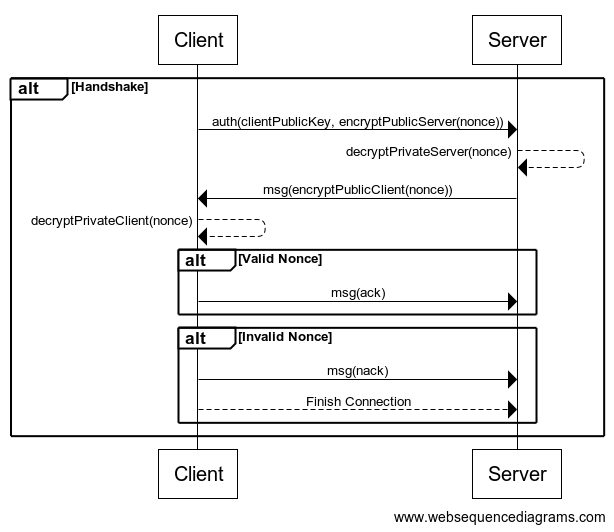
\includegraphics[width=0.7\textwidth]{diagrama/handshake.png}}
    \caption{Etapa de Handshake}
    \label{fig:handshake}
    \end{figure}
    
    \subsection{Generate Symmetric Key}
    \begin{itemize}
    \item A segunda etapa é iniciada pelo \textbf{Server}, que gera a chave simétrica, a ser compartilhada com o \textbf{Client} na conexão individual. Após gerar sua chave simétrica, o \textbf{Server} enviará um pacote ao \textbf{Client} chamado \textbf{msg}. Tal pacote possui um único parâmetro cujo valor é chave simétrica previamente encriptada pela chave pública do \textbf{Client}. Essa encriptação é feita por meio da função \textit{encryptPublicClient(symmetricKey)}.
    \end{itemize}
    
    \begin{figure}[ht]
    \centerline{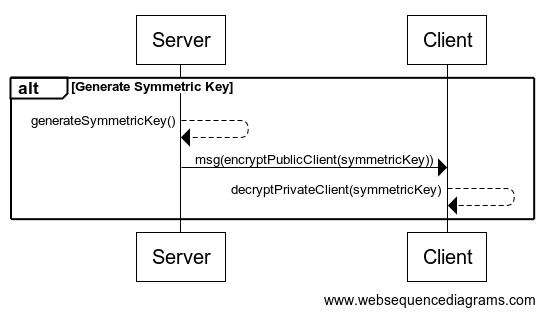
\includegraphics[width=0.7\textwidth]{diagrama/generateSymmetric.png}}
    \caption{Etapa de Generate Symmetric Key}
    \label{fig:symmetric}
    \end{figure}
    
    \subsection{Vote Session}
    \begin{itemize}
    \item Dentro da terceira etapa, existe um loop, no qual o \textbf{Client} enviará um pacote chamado \textbf{vote}, que possui um único parâmetro cujo valor é a pessoa votada, previamente encriptada através da chave simétrica (isso é feito pela função \textit{encryptSymmetric}).
    \item Após as validações do voto (nas etapas de desencriptação), se ele for considerado um voto válido é enviado um pacote \textbf{msg} do \textbf{Server} para o \textbf{Client} que possui um único parâmetro que é uma mensagem \textit{ack} encriptada através da função \textit{encryptSymmetric}.
    \item Em caso contrário (voto inválido), é enviado um pacote \textbf{msg} do \textbf{Server} para o \textbf{Client} que possui um único parãmetro que é uma mensagem \textit{nack} encriptada através da função \textit{encryptSymmetric}.
    \end{itemize}
    
    \begin{figure}[ht]
    \centerline{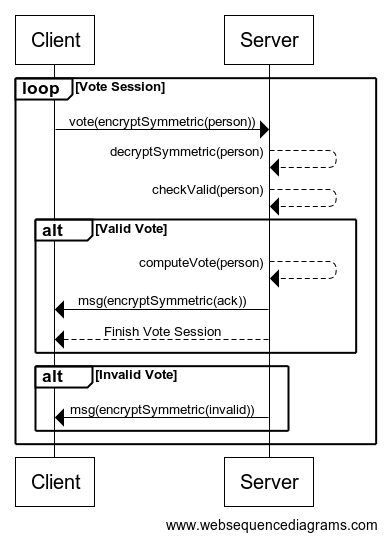
\includegraphics[width=0.7\textwidth]{diagrama/voteSession.png}}
    \caption{Etapa de Vote Session}
    \label{fig:voteSession}
    \end{figure}
    
\section{Garantia dos Requisitos de Segurança}
    \begin{itemize}
    \item A presente seção tem como objetivo descrever como a autenticidade e a confidencialidade são garantidas através do protocolo desenvolvido.
    \end{itemize}
    
    \subsection{Autenticidade}
    \begin{itemize}
    \item Pensamos em garantir apenas a autenticidade do \textbf{Server}, já que ele é, basicamente, o responsável pelo processo de votação.
    \item Para que esse processo fosse possível, assumimos que a \textit{public key} do \textbf{Server} estará disponível com antecedência para todos os \textbf{Clients} na rede. Dessa forma, inicialmente, o \textbf{Client} envia um pacote para o \textbf{Server} iniciando a comunicação, no qual os parâmetros enviados são a \textit{public key} do \textbf{Client}, que está se comunicando, e um \textit{nonce} (string aleatória), que é criptografado com a \textit{public key} do \textbf{Server}.
    \item É esperado, portanto, que o \textbf{Server} possua a \textit{private key} e que, com ela, possa desencriptar o pacote contendo o \textit{nonce} e obter seu valor.
    \item Para finalmente estabelecer a conexão, é necessário que o \textbf{Server} envie para o \textbf{Client} uma mensagem contendo o mesmo \textit{nonce} recebido só que desta vez encriptado com a \textit{public key} do \textbf{Client}, que foi obtida no primeiro pacote da conversação.
    \item O \textbf{Client} então irá realizar o mesmo processo de desencriptação com a sua \textit{private key} e, se o valor do \textit{nonce} desencriptado corresponder ao valor do \textit{nonce} enviado, assumimos então que o \textbf{Server} é autêntico e prosseguimos com a conexão.
    \end{itemize}
    
    \subsection{Confidencialidade}
    \begin{itemize}
    \item Após a etapa de \textit{handshake}, o \textbf{Server} irá gerar uma chave simétrica por meio da função \textit{generateSymmetricKey} e enviará um pacote \textbf{msg}, que contém essa chave simétrica encriptada pela \textit{public key} do \textbf{Client}. 
    \item Recebido o pacote, o \textbf{Client} irá desencriptá-lo com sua \textit{private key} e obterá a chave simétrica. Feito isso, o \textbf{Client} iniciará a etapa de \textit{Vote Session} enviando o pacote \textbf{vote}, que contém a sua escolha de voto encriptada pela chave simétrica.
    \item Perceba que, a chave simétrica é primeiro encriptada pela \textit{public key} do \textbf{Client} antes de ser enviada. Sendo assim, ela só pode ser descoberta por meio de uma desencriptação usando a \textit{private key} desse mesmo \textbf{Client}. Como apenas o \textbf{Client} em si possui acesso a sua \textit{private key}, não é possível que um atacante consiga descobrir nem a \textit{private key} do \textbf{Client} e nem a chave simétrica, garantindo assim a confidencialidade do voto.
    \item Após isso, é feita no \textbf{Server} uma etapa de validação do voto e independente do voto ser válido ou não, é enviado um pacote \textbf{msg} contendo o status do voto (válido ou inválido) encriptado pela chave simétrica compartilhada anteriormente. Isso assegura que um possível atacante não será capaz de saber se um voto foi de fato computado ou não.
     \end{itemize}
    
\section{A Biblioteca}
    \begin{itemize}
    \item Para que a biblioteca desenvolvida possa ser utilizada em uma aplicação qualquer, é necessário adicionar o arquivo "protocol.py" ao projeto da aplicação desenvolvida em Python.
    \item Para fazer uso da biblioteca, deve-se adicionar a linha: \texttt{import protocol} no início de cada arquivo ".py" que fará uso das funcionalidades da biblioteca.
    \item Como a biblioteca desenvolvida faz uso de outros pacotes de terceiros, é necessário instalar alguns deles por meio do terminal, como será explicado abaixo.
    \end{itemize}

\section{Dependências}
    \begin{itemize}
    \item A biblioteca desenvolvida faz uso de outros pacotes, necessários para auxiliar na implementação de certas funcionalidades da biblioteca. Seu uso se faz necessário principalmente na criptografia presente no protocolo desenvolvido. Os pacotes utilizados foram:
    \begin{enumerate}
        \textbf{\item os}
        \textbf{\item socket}
        \textbf{\item ast}
        \textbf{\item random}
        \textbf{\item collections}
        \textbf{\item base64}
        \textbf{\item Crypto} (Esse pacote específico deve ser instalado por meio do comando: “pip3 install pycryptodome” no terminal). A documentação desse pacote em particular pode ser encontrada em: https://pycryptodome.readthedocs.io/en/latest/index.html
    \end{enumerate}
    \end{itemize} 
    
\section{Estrutura}
    \begin{itemize}
    \item A biblioteca desenvolvida foi estruturada de forma que possui 5 classes distintas, que implementam, de forma modularizada, as características do protocolo previamente descritas. 
    \item As classes em questão são: \textbf{bcolors}, \textbf{Socket}, \textbf{Server}, \textbf{Client} e \textbf{Protocol}.
    \item Por questões de organização, a estrutura foi pensada de forma hierárquica, de maneira que existem superclasses e subclasses na biblioteca. A hierarquia mencionada pode ser vista abaixo:
    
    \begin{figure}[ht]
    \centering{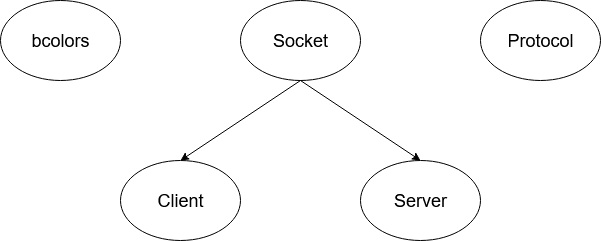
\includegraphics[scale=0.35]{ClassHierarchy.png}}
    \caption{Hierarquia da Biblioteca}
    \label{fig:diagrama}
    \end{figure}
    
    \item Iniciaremos agora a descrição de cada uma das classes, passando por seu objetivo, seus atributos e seus métodos.

    \subsection{\Large bcolors}
        \subsubsection{\large Objetivo}
            \begin{itemize}
            \item A classe tem como objetivo agrupar uma série de códigos de cores e de modificadores de
            texto, de forma que as mensagens geradas pela biblioteca possam ser visualizadas mais
            facilmente no terminal pelos usuários, caso seja necessário.
            \end{itemize}
        \subsubsection{\large Atributos}
            \begin{itemize}
            \item \textbf{bcolors.HEADER:} Atributo responsável por guardar o código responsável por realizar a alteração no texto presente no terminal para o formato cabeçalho/header. \texttt{Tipo: str.} 
            \item \textbf{bcolors.OKBLUE:} Atributo responsável por guardar o código referente à cor Azul. O atributo é utilizado para emitir mensagens de sucesso pela biblioteca. \texttt{Tipo: str.}
            \item \textbf{bcolors.OKCYAN:} Atributo responsável por guardar o código referente à cor Ciano. O atributo é utilizado para emitir mensagens de sucesso pela biblioteca. \texttt{Tipo: str.}
            \item \textbf{bcolors.OKGREEN:} Atributo responsável por guardar o código referente à cor Verde. O atributo é utilizado para emitir mensagens de sucesso pela biblioteca. \texttt{Tipo: str.}
            \item \textbf{bcolors.WARNING:} Atributo responsável por guardar o código utilizado quando é preciso emitir uma mensagem de aviso/warning. \texttt{Tipo: str.}
            \item \textbf{bcolors.FAIL:} Atributo responsável por guardar o código referente à cor Vermelho. O atributo é utilizado para emitir mensagens de erro/fail pela biblioteca. \texttt{Tipo: str.}
            \item \textbf{bcolors.ENDC:} Atributo responsável por guardar o código que indica que não serão usados outros atributos para modificar a mesma string em questão. Ele sempre é utilizado após o final da string. \texttt{Tipo: str.}
            \item \textbf{bcolors.BOLD:} Atributo responsável por guardar o código responsável por realizar a alteração no texto presente no terminal para o formato negrito/bold. \texttt{Tipo: str.} 
            \item \textbf{bcolors.UNDERLINE:} Atributo responsável por guardar o código responsável por realizar a alteração no texto presente no terminal para o formato sublinhado/underline. \texttt{Tipo: str.} 
            \end{itemize}
        \subsubsection{\large Métodos}
            \begin{itemize}
            \item Não há métodos nessa classe.
            \end{itemize}
        
    \subsection{\Large Socket}
        \subsubsection{\large Objetivo}
            \begin{itemize}
            \item A classe tem como objetivo não só criar um socket para que a comunicação entre cliente e servidor ocorra, mas também implementar algumas funcionalidades de criptografia necessárias para o funcionamento adequado do protocolo desenvolvido.
            \end{itemize}
        \subsubsection{\large Atributos}
            \begin{itemize}
            \item \textbf{Socket.socket:} Esse atributo é responsável por guardar o objeto \texttt{socket.socket}, criado no construtor dessa classe e presente no módulo “socket”. \texttt{Tipo: socket.socket.}
            \item \textbf{Socket.address:}  Esse atributo é responsável por armazenar o endereço IP referente ao hospedeiro em questão. \texttt{Tipo: str.} 
            \item \textbf{Socket.port:} Esse atributo é responsável por armazenar o número de porta referente ao socket criado no hospedeiro em questão. \texttt{Tipo: str.}
            \item \textbf{Socket.publicKey:} Esse atributo é responsável por armazenar a chave pública do socket no hospedeiro em questão. \texttt{Tipo: Crypto.PublicKey.RSA.RsaKey.}
            \item \textbf{Socket.privateKey:} Esse atributo é responsável por armazenar a chave privada do socket no hospedeiro em questão. \texttt{Tipo: Crypto.PublicKey.RSA.RsaKey.}
            \end{itemize}
        \subsubsection{\large Métodos}
            \begin{itemize}
            \item \textbf{Socket(address, port):} Esse método é o construtor da classe. O método possui como parâmetros: \underline{address} (O endereço IP do hospedeiro no qual o socket foi criado. \texttt{Tipo: str}) e \underline{port} (O número de porta a ser usado pelo socket. \texttt{Tipo: str}). O método retorna um objeto do \texttt{tipo: protocol.Socket.}
            \item \textbf{Socket.connect():} Esse método é responsável por realizar a conexão de um hospedeiro
            com outro. Uma vez que a forma como a conexão é executada varia de cliente para servidor, essa implementação está vazia e a implementação de fato desse método está presente nas subclasses da classe “Socket”: classe “Client” e classe “Server”. Em outras palavras, esse método funciona como um método abstrato. O método não possui nenhum parâmetro e não retorna nada.
            \item \textbf{Socket.generateAsymmetricKeys():} Esse método é responsável por gerar as chaves assimétricas (chave privada e chave pública) do socket no hospedeiro em questão. Tanto a chave privada como a chave pública são geradas com o auxílio do pacote “Crypto” mencionado anteriormente. Além disso, é executado automaticamente quando o construtor da classe “Socket” é chamado. O método não possui nenhum parâmetro e não retorna nada.
            \item \textbf{Socket.encryptMessage(message, key, encryptType="asymmetric"):} Esse \newline método é responsável por realizar a encriptação de uma mensagem fornecida, dada uma chave e um modo de encriptação. Perceba que o último parâmetro é opcional e, por padrão, será usado o modo de encriptação “asymmetric”. O método possui os seguintes parâmetros: \underline{message} (A mensagem a ser encriptada. \texttt{Tipo: bytearray}), \underline{key} (A chave a ser usada na encriptação. \texttt{Tipo: Crypto.PublicKey.RSA.RsaKey}) e \underline{encryptType} (O modo de encriptação a ser usado. \texttt{Tipo: str}. Esse parâmetro pode possuir apenas dois valores: “symmetric” ou “asymmetric”). O método pode retornar dois tipos de objetos dependendo de qual modo de encriptação foi usado. Se foi usado o modo de encriptação “asymmetric”, o método retorna um objeto \texttt{tipo: bytes.} Por outro lado, se foi usado o modo de encriptação “symmetric”, o método retorna um objeto \texttt{tipo: dict.}
            \item \textbf{Socket.decryptMessage(message, key, encryptType="asymmetric", iv=“‘‘):} Esse método é responsável por realizar a desencriptação de uma mensagem fornecida, dada uma chave, um modo de encriptação e um iv/vetor de inicialização. Perceba que os dois últimos parâmetros são opcionais e, por padrão, será utilizado o modo de encriptação “asymmetric” e o iv terá o valor: “”. O método possui os seguintes parâmetros: \underline{message} (A mensagem a ser encriptada. \texttt{Tipo: bytearray}), \underline{key} (A chave a ser usada na desencriptação. \texttt{Tipo: Crypto.PublicKey.RSA.RsaKey}), \underline{encryptType} (O modo de desencriptação a ser usado. \texttt{Tipo: str}. Esse parâmetro pode possuir apenas dois valores: “symmetric” ou “asymmetric”) e \underline{iv} (O vetor de inicialização a ser usado, caso o modo de encriptação seja “symmetric”. \texttt{Tipo: bytes}). O método retorna apenas um tipo de objeto, independente de qual modo de encriptação foi usado. O método retorna um objeto \texttt{tipo: bytes}.
            
            \end{itemize}
        
    \subsection{\Large Server}
        \subsubsection{\large Objetivo}
            \begin{itemize}
            \item A classe tem com objetivo representar o estado e o comportamento de um servidor, conforme apresentado previamente na descrição do protocolo. Como descrito em seções anteriores, o protocolo desenvolvido separa as funcionalidades do cliente e do servidor em classes distintas. Além disso, ambas as classes mencionadas são subclasses da classe "Socket" descrita acima.
            \end{itemize}
        \subsubsection{\large Atributos}
            \begin{itemize}
            \item Por ser uma subclasse da classe "Socket", a classe "Server" possui todos os atributos da classe "Socket" descritos previamente. Ademais, possui os seguintes atributos específicos da própria classe "Server":
            \item \textbf{Server.candidates:}  Esse atributo é responsável por guardar a lista com todas as opções válidas de candidatos na votação. \texttt{Tipo: list}.
            \item \textbf{Server.votes:} Esse atributo é responsável por contabilizar os votos de todas as opções válidas de candidatos na votação. \texttt{tipo: dict}.
            \end{itemize}
        \subsubsection{\large Métodos}
            \begin{itemize}
            \item Por ser uma subclasse da classe "Socket", a classe "Server" possui todos os métodos da classe "Socket" descritos previamente. Ademais, possui os seguintes métodos específicos da própria classe "Server":
            \item \textbf{Server(address, port, candidates):} : Esse método é o construtor da classe. Nesse construtor, ocorre a chamada do método responsável por gerar as chaves assimétricas (chave pública e chave privada) e, além disso, a chave pública do servidor será armazenada em um arquivo do tipo "txt" cujo nome é: "serverPublicKey.txt". O método possui como parâmetros: \underline{address} (O endereço IP do servidor. \texttt{Tipo: str}), \underline{port} (O número de porta a ser usado pelo socket do servidor. \texttt{Tipo: str}) e \underline{candidates} (A lista de opções válidas de candidatos na eleição. \texttt{Tipo: list}). O método retorna um objeto do \texttt{tipo: protocol.Server}.
            \item \textbf{Server.connect():} : Esse método é responsável por criar a ligação do socket do servidor com um endereço e porta. Em seguida, ele faz com que o socket do servidor “escute” por novas conexões. O método não possui nenhum parâmetro e não retorna nada.
            \item \textbf{Server.sendMessage(clientSocket, message):} Esse método é responsável por enviar uma mensagem a um cliente específico. O método possui como parâmetros: \underline{clientSocket} (O socket do cliente para o qual a mensagem proveniente do servidor será enviada. \texttt{Tipo: socket.socket}) e \underline{message} (A mensagem que será enviada para o socket do cliente em questão. \texttt{Tipo: bytes}). O método não retorna nada.
            \item \textbf{Server.checkValidCandidate(candidate):}  Esse método é responsável por verificar se um candidato recebido é, de fato, uma opção válida de voto. O método possui um único parâmetro: \underline{candidate} (Um nome representando o candidato votado. \texttt{Tipo: str}). O método retorna um booleano (\texttt{tipo: bool}), indicando se a opção fornecida é válida ou não.
            \item \textbf{Server.addVote(candidate):} Esse método é responsável por computar o voto referente a uma opção de candidato, que já foi verificada e apontada como válida. O método possui como único parâmetro: \underline{candidate} (Um nome representando o candidato votado. \texttt{Tipo: str}). O método não retorna nada.
            \item \textbf{Server.printVotes():} Esse método é responsável por imprimir na tela do terminal todas as opções válidas de candidatos e a quantidade respectiva dos seus votos computados até o momento da chamada do método. Esse método não possui nenhum parâmetro e não retorna nada.
            \end{itemize}
        
    \subsection{\Large Client}
        \subsubsection{\large Objetivo}
            \begin{itemize}
            \item A classe tem com objetivo representar o estado e o comportamento do cliente, conforme apresentado previamente na descrição do protocolo. Como descrito em seções anteriores, o protocolo desenvolvido separa as funcionalidades do cliente e do servidor em classes distintas. Além disso, ambas as classes mencionadas são subclasses da classe "Socket" descrita anteriormente.
            \end{itemize}
        \subsubsection{\large Atributos}
            \begin{itemize}
            \item Por ser uma subclasse da classe "Socket", a classe "Client" possui todos os atributos da classe "Socket" descritos previamente. No entanto, a classe "Client" não possui atributos específicos próprios dela mesma.
            \end{itemize}
        \subsubsection{\large Métodos}
            \begin{itemize}
            \item Por ser uma subclasse da classe "Socket", a classe "Client" possui todos os métodos da classe "Socket" descritos previamente. Ademais, possui os seguintes métodos específicos da própria classe "Client":
            \item \textbf{Client(address, port):} Esse método é o construtor da classe. O método possui como parâmetros: \underline{address} (O endereço IP do servidor ao qual o cliente deve se conectar. \texttt{Tipo: str}) e \underline{port} (O número de porta utilizado pelo socket do servidor ao qual o cliente irá se conectar. \texttt{Tipo: str}).  O método retorna um objeto do \texttt{tipo: protocol.Client}.
            \item \textbf{Client.connect():} Esse método é responsável por criar uma conexão entre o cliente em questão e o (socket do) servidor. O método não possui nenhum parâmetro e não retorna nada.
            \item \textbf{Client.sendMessage(message):} Esse método é responsável por enviar uma mensagem do cliente para o servidor. O método possui um único parâmetro: \underline{message} (A mensagem que será enviada do cliente para o servidor. \texttt{Tipo: bytes}). O método não retorna nada.
            \end{itemize}
        
    \subsection{\Large Protocol}
        \subsubsection{\large Objetivo}
            \begin{itemize}
            \item A classe tem como objetivo implementar, de forma sequencial e modularizada, as etapas do protocolo descritas na entrega anterior (etapa de "Handshake", etapa de geração de chave simétrica e etapa de sessão de votação). Para isso, como será explicado adiante, existe uma divisão entre as atividades executadas pelo cliente em todas as etapas e as atividades executadas pelo servidor em todas as etapas.
            \end{itemize}
        \subsubsection{\large Atributos}
            \begin{itemize}
            \item \textbf{Protocol.symmetricKey:}  Esse atributo é responsável por armazenar a chave simétrica, que será compartilhada entre a conexão individual cliente-servidor. \texttt{Tipo: bytes}.
            \end{itemize}
        \subsubsection{\large Métodos}
            \begin{itemize}
             \item \textbf{Protocol():} Esse método é o construtor da classe. O método não possui nenhum parâmetro. O método retorna um objeto do \texttt{tipo: protocol.Protocol}.
             \item \textbf{Protocol.generateRandomKey():} Esse método é responsável pela geração, de forma aleatória, da chave simétrica que será compartilhada na conexão individual cliente-servidor. O método não possui nenhum parâmetro e retorna um objeto do \texttt{tipo: bytes}.
             \item \textbf{Protocol.clientProcedure(client, serverPublicKey):} Esse método é responsável por executar, de forma sequencial, todas as atividades atribuídas ao cliente nas duas primeiras etapas do protocolo definidas anteriormente. Ou seja, o método executa as funções do cliente nas etapas de: "Handshake" e geração de chave simétrica, respectivamente. O método possui como parâmetros: \underline{client} (O cliente que está interagindo/conectado com o servidor. \texttt{Tipo: protocol.Client}) e \underline{serverPublicKey} (A chave pública do servidor, que é assumida ser de conhecimento geral. \texttt{tipo: Crypto.PublicKey.RSA.RsaKey}). O método não retorna nada.
             \item \textbf{Protocol.clientVote(client, votedPerson, serverPublicKey):} Esse método é responsável por executar as atividades atribuídas ao cliente na última etapa do protocolo (etapa de sessão de votação). O método possui como parâmetros: \underline{client} (O cliente que está interagindo/conectado com o servidor. \texttt{Tipo: protocol.Client}), \underline{votedPerson} (Um nome indicando o candidato votado. \texttt{Tipo: str}) e \underline{serverPublicKey} (A chave pública do servidor, que é assumida ser de conhecimento geral. \texttt{tipo: Crypto.PublicKey.RSA.RsaKey}). O método não retorna nada.
             
             \item \textbf{Protocol.serverProcedure(server, clientSocket, clientAddress):} Esse método é responsável por executar, de forma sequencial, todas as atividades atribuídas ao servidor nas etapas do protocolo definidas anteriormente. Ou seja, o método executa as funções do servidor nas etapas de: "Handshake", geração de chave simétrica e sessão de votação, respectivamente. O método possui como parâmetros: \underline{server} (O servidor que está executando o seu procedimento no protocolo. \texttt{Tipo: protocol.Server}), \underline{clientSocket} (O socket do cliente com o qual o servidor em questão está conectado. \texttt{Tipo: socket.socket}) e \underline{clientAddress} (Uma tupla contendo o endereço IP do cliente e o número de porta utilizado pelo socket desse mesmo cliente ao qual o servidor está conectado. \texttt{Tipo: tuple}). O método não retorna nada.
             
            \end{itemize}
    \end{itemize}
\end{document}